\chapter{Implementacija i korisničko sučelje}
		
		
		\section{Korištene tehnologije i alati}
		
		Komunikacija u timu je ostvarena putem korištenja aplikacije WhatsApp\footnote{\url{https://www.whatsapp.com/}}. Komunikacija sa asistentom ostvarena je korištenjem aplikacije Microsoft Teams\footnote{\url{https://www.microsoft.com/hr-hr/microsoft-teams/group-chat-software/}}. Za izradu dijagrama korišten je Astah Professional\footnote{\url{https://astah.net/products/astah-professional/}}. Za upravljanje izvornim kodom korišten je alat Git\footnote{\url{https://git-scm.com/}}. Udaljeni repozitorij projekta nalazi se na platformi GitHub\footnote{\url{https://github.com/}}.
		
		Kao razvojno okruženje na backendu korišten je IntelliJ\footnote{\url{https://www.jetbrains.com/idea/}}, a na frontendu Visual Studio Code\footnote{\url{https://code.visualstudio.com/}}. Visual Studio Code je razvojno okruženje tvrtke Microsoft za Windows, Linux, macOS. Za razvoj softvera koristi Microsoftove platforme poput Windows API, Windows Forms, Windows Presentation Foundation, Windows Store i Microsoft Silverlight.
		
		Tehnologije korištene za razvoj backenda su Spring Boot\footnote{\url{https://spring.io/projects/spring-boot}} i programski jezik Java\footnote{\url{https://www.java.com/en/}}. Tehnologije korištene za razvoj frontenda su Angular\footnote{\url{https://angular.io/}} i programski jezik TypeScript\footnote{\url{https://www.typescriptlang.org/}}. Angular je besplatni okvir(framework) za izgradnju web aplikacija otvorenog izvornog koda temeljen na TypeScriptu. Angular se temelji na principu komponenata gdje nekoliko nezavisnih komponenti surađuje kako bi oblikovali korisničko sučelje. Takva struktura čini aplikacije lako prilagodljivim i održivim.
		
		Za automatizirano testiranje koristen je alat Selenium IDE\footnote{\url{https://www.selenium.dev/documentation/ide/}}. Za puštanje aplikacije u pogon korištena je platforma Render\footnote{\url{https://render.com/}}.
		
		Baza podataka zadužena za pohranu podataka je PostgreSQL\footnote{\url{https://www.postgresql.org/}}.
		
		
	
	
	
		\section{Ispitivanje programskog rješenja}
			
			\textbf{\textit{dio 2. revizije}}\\
			
			 \textit{U ovom poglavlju je potrebno opisati provedbu ispitivanja implementiranih funkcionalnosti na razini komponenti i na razini cijelog sustava s prikazom odabranih ispitnih slučajeva. Studenti trebaju ispitati temeljnu funkcionalnost i rubne uvjete.}
	
			
			\subsection{Ispitivanje komponenti}
			\textit{Potrebno je provesti ispitivanje jedinica (engl. unit testing) nad razredima koji implementiraju temeljne funkcionalnosti. Razraditi \textbf{minimalno 6 ispitnih slučajeva} u kojima će se ispitati redovni slučajevi, rubni uvjeti te izazivanje pogreške (engl. exception throwing). Poželjno je stvoriti i ispitni slučaj koji koristi funkcionalnosti koje nisu implementirane. Potrebno je priložiti izvorni kôd svih ispitnih slučajeva te prikaz rezultata izvođenja ispita u razvojnom okruženju (prolaz/pad ispita). }
			
			
			
			\subsection{Ispitivanje sustava}
			
			 \textit{Potrebno je provesti i opisati ispitivanje sustava koristeći radni okvir Selenium\footnote{\url{https://www.seleniumhq.org/}}. Razraditi \textbf{minimalno 4 ispitna slučaja} u kojima će se ispitati redovni slučajevi, rubni uvjeti te poziv funkcionalnosti koja nije implementirana/izaziva pogrešku kako bi se vidjelo na koji način sustav reagira kada nešto nije u potpunosti ostvareno. Ispitni slučaj se treba sastojati od ulaza (npr. korisničko ime i lozinka), očekivanog izlaza ili rezultata, koraka ispitivanja i dobivenog izlaza ili rezultata.\\ }
			 
			 \textit{Izradu ispitnih slučajeva pomoću radnog okvira Selenium moguće je provesti pomoću jednog od sljedeća dva alata:}
			 \begin{itemize}
			 	\item \textit{dodatak za preglednik \textbf{Selenium IDE} - snimanje korisnikovih akcija radi automatskog ponavljanja ispita	}
			 	\item \textit{\textbf{Selenium WebDriver} - podrška za pisanje ispita u jezicima Java, C\#, PHP koristeći posebno programsko sučelje.}
			 \end{itemize}
		 	\textit{Detalji o korištenju alata Selenium bit će prikazani na posebnom predavanju tijekom semestra.}
			
			\eject 
		
		
		\section{Dijagram razmještaja}
			
			Na slici 5.1 nalazi se dijagram razmještaja. Dijagram razmještaja prikazuje fizičku strukturu programskog sustava. Glavna svrha mu je pobliže prikazati arhitekturu razmještaja sustava. Korisnici pristupaju aplikaciji korištenjem web preglednika. Komunikacija se odvija putem protokola HTTP. Na platformi Render se nalaze poslužitelji za frontend, backend i bazu podataka.
			
			\begin{figure}[H]
				\centering
				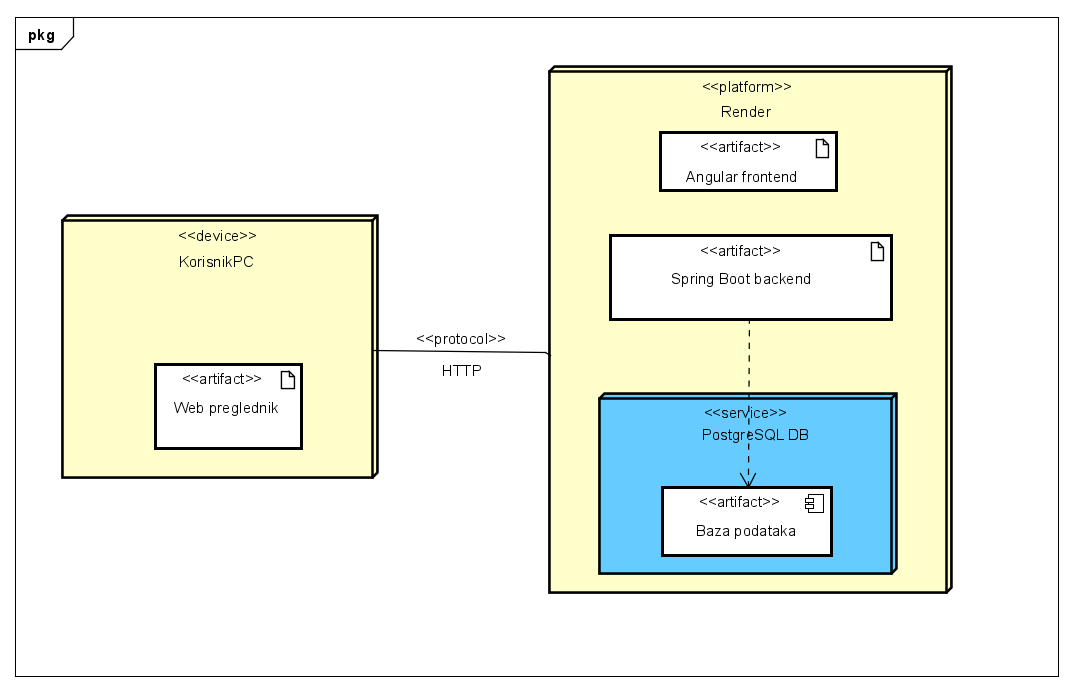
\includegraphics[width=\textwidth]{slike/Dijagram_razmjestaja.PNG}
				\caption{Dijagram razmještaja }
				\label{fig:dijagram_baze}
			\end{figure}
			
		\vspace{108pt}
		
		
		\section{Upute za puštanje u pogon}
		
			\textbf{\textit{dio 2. revizije}}\\
		
			 \textit{U ovom poglavlju potrebno je dati upute za puštanje u pogon (engl. deployment) ostvarene aplikacije. Na primjer, za web aplikacije, opisati postupak kojim se od izvornog kôda dolazi do potpuno postavljene baze podataka i poslužitelja koji odgovara na upite korisnika. Za mobilnu aplikaciju, postupak kojim se aplikacija izgradi, te postavi na neku od trgovina. Za stolnu (engl. desktop) aplikaciju, postupak kojim se aplikacija instalira na računalo. Ukoliko mobilne i stolne aplikacije komuniciraju s poslužiteljem i/ili bazom podataka, opisati i postupak njihovog postavljanja. Pri izradi uputa preporučuje se \textbf{naglasiti korake instalacije uporabom natuknica} te koristiti što je više moguće \textbf{slike ekrana} (engl. screenshots) kako bi upute bile jasne i jednostavne za slijediti.}
			
			
			 \textit{Dovršenu aplikaciju potrebno je pokrenuti na javno dostupnom poslužitelju. Studentima se preporuča korištenje neke od sljedećih besplatnih usluga: \href{https://aws.amazon.com/}{Amazon AWS}, \href{https://azure.microsoft.com/en-us/}{Microsoft Azure} ili \href{https://www.heroku.com/}{Heroku}. Mobilne aplikacije trebaju biti objavljene na F-Droid, Google Play ili Amazon App trgovini.}
			
			
			\eject 